\chapter{Historia}

\section{Antecedentes}

\noindent Las primeras formas fractales aparecieron en el siglo XIX, cuando el matemático Karl Weierstrass graficó en 1872 su famosa función de Weierstrass. Más tarde en ese mismo siglo, empezaron a surgir conceptos cada vez más cercanos a lo que hoy se consideran fractales, siendo más gemométricos y menos algebraicos.

\begin{figure}[H]
    \centering
    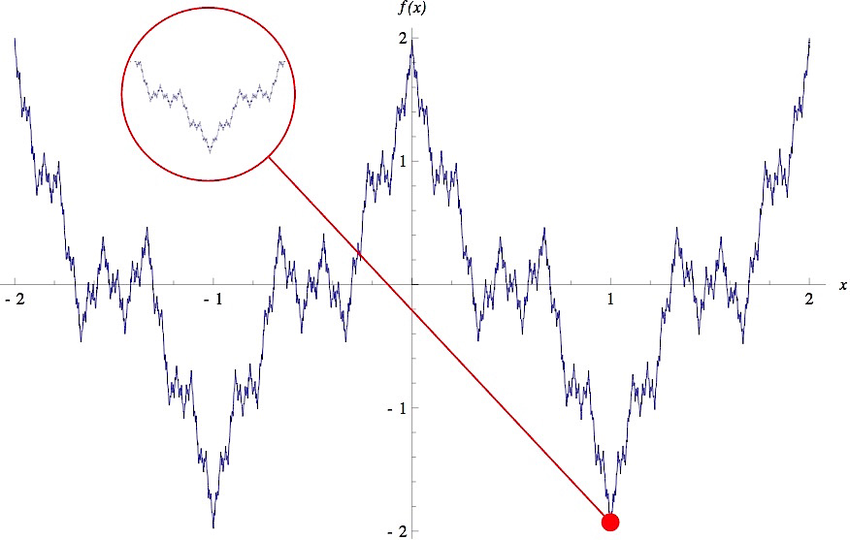
\includegraphics[width=0.5\textwidth]{figures/weierstrass-function.png}
    \caption{Función de Weierstrass}
    \label{fig:weierstrass-function}
\end{figure}

\section{Primeros fractales}

\noindent Así, en 1904, Helge von Koch definió su copo de nieve, una curva con propiedades similares a la de Weierstrass. En 1915, Waclaw Sierspinski construyó su triángulo y, un año después, su alfombra.

\begin{figure}[H]
    \centering
    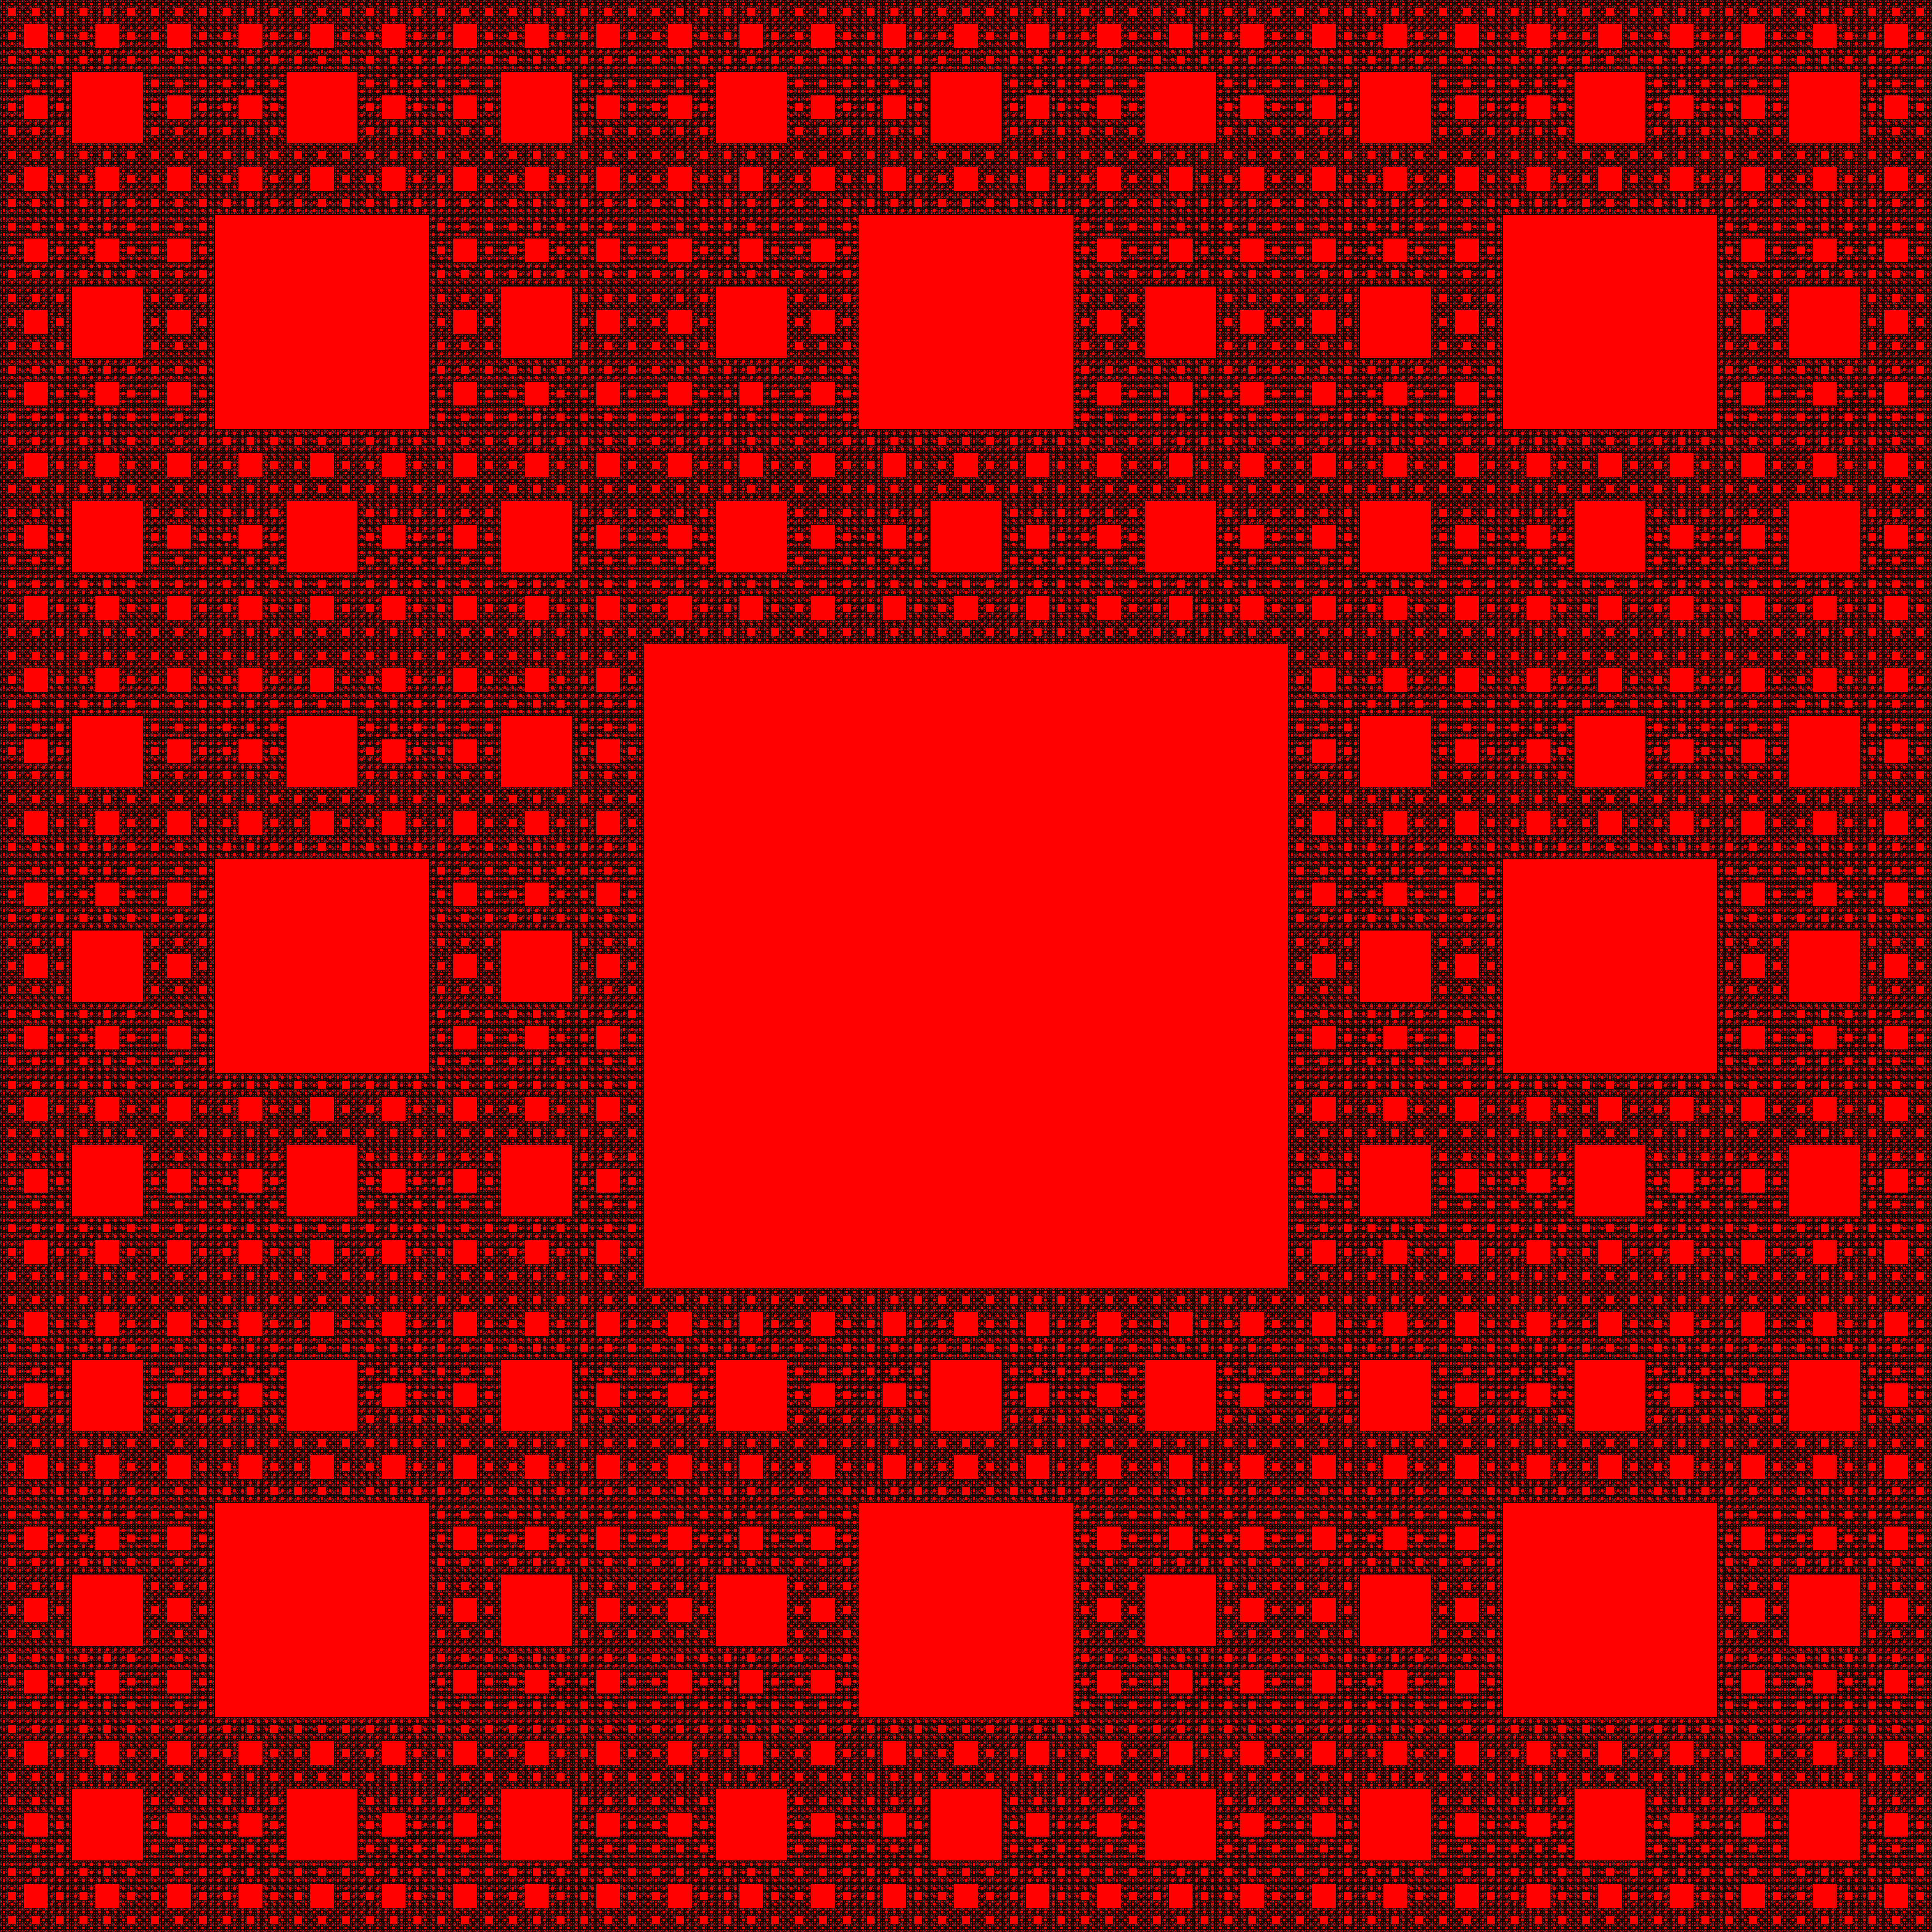
\includegraphics[width=0.5\textwidth]{figures/sierspinsky-carpet.png}
    \caption{Alfombra de Sierspinsky}
    \label{fig:sierspinsky-carpet}
\end{figure}